\chapter{Reinforcement Learning}\label{chap:reinforcement}

\chapterQuote{
    \textit{``Caminante, no hay camino, se hace camino al andar.''}\\
    \textit{(``Traveler, there is no path, you make your path as you walk.'')}
    }{--- Antonio Machado}

\chapterAbstract{A}{qui hablamos tanto del RL de base y su historia y como funciona hasta de como se plaica en los grafos de conocimiento y porque provee de un razonamiento intrinseco.

Mencionamos tambien metodologia de los diferentes algoritmos como PPO, SAC, reinforce vs Actor critic etc etc...}

\section{Introduction}\label{sec:rl-intro}
An explanation of how reinforcement learning works and where its usefull.
% A relational path is a sequence of relations that connect two entities together in a Knowledge Graph. There can be many such paths between any two entities, and they can vary in length and complexity. Given that these paths can provide an interesting insight on how related two entities are, many researchers have developed methods to analyze them to learn what constitutes correct knowledge. 

% Generally, these methods generate features that characterize the information contained in each path, and then train classifiers to predict the existence of missing relations based on these features. Due to the high number of possible paths that can exist between two entities, such methods usually use techniques like random walks to restrict the amount of paths that are analyzed, possibly constraining their effectiveness.

% To solve this issue, other methods analyze graph neighborhoods, which refer to the entities and relationships that are directly connected to a given entity in a Knowledge Graph. This allows KG completion method to focus on a much more reduced amount of information that is more likely to accurately characterize an entity.

% In this chapter, we present an overview on the methods that rely on these techniques to complete a Knowledge Graph. We first introduce the methods that rely purely on relational paths and their characterization. Next, we present the methods that analyze entity neighborhoods. Finally, we discuss more advanced methods that combine these approaches with techniques from the previous chapter.

\section{Algorithms}\label{sec:rl-algorithms}
We categorize and evaluate the different algorithms and progress that has been made in the field of reinforcement learning 

% A relational path is simply a concatenation of triples that connect an entity to some other entity through a number of relations. Naturally, any Knowledge Graph has an abundance of possible paths to, from, or between entities. The idea of analyzing such paths to learn what constitutes valid knowledge has led to many research works.

% One of the first approaches that exploited relational paths in a Knowledge Graph was the Path Ranking Algorithm (PRA), proposed by \citet{lao2011}. PRA uses random walks to generate a set of paths between a given pair of entities in a depth-first manner. The generated paths are then transformed into a series of features that aim to characterize the information contained in it. These features are ultimately used to train a binary log-linear classifier, which learns whether a direct relationship should exist between two entities according to the paths that are already present between them. However, PRA is not without limitations. The number of possible paths between a pair of entity can be very high, limiting its scalability. Additionally, the randomly guided paths that it uses may miss information just by mere chance.

% Aiming to improve PRA, \citet{gardner2015} introduced the Subgraph Feature Extraction (SFE) method. In opposition to PRA, SFE uses a breadth-first search that is not randomly guided, in order to better characterize the portion of the KG between two entities. SFE also requires the creation of a handmade ``Alias'' relation, which relates entities in the same KG that refer to the same element in the real world. It is able to achieve more expressive results than PRA, making it easier for the human user to understand what constitutes a good path that may be indicative of the existence of a direct relation between two entities.

% \citet{gardner2013} also proposed an extension of PRA that addresses the issue of potentially having to consider a very high number of paths. It considers the semantic similarities between the relations of a Knowledge Graph, and uses them to merge very similar paths together, greatly reducing the number of paths that need to be analyzed afterwards. This addition increases the effectivity of PRA in the NELL Knowledge Graph, although the authors do not provide data for any other KGs.

% \citet{nastase2019} proposed the Abstract Path Model (APM), which produces an abstract graph from a KG, and then focuses on extracting relevant abstract paths from it. These abstract graphs provide a more general representation of the high-level relations between entities, and thus the paths that can be traced in it represent more high-level knowledge. Additionally, this abstract representation is, as a general rule, considerably smaller than the KG it is derived from and not very computationally taxing to obtain, which aids in its application to larger graphs.

% \citet{gu2015} introduced the Trans-COMP method, which proposes a different strategy. Rather than analyzing a large number of paths between two entities to try to characterize the pair, it only uses a single path. Precisely, it aims to select the path that provides the highest predictive capabilities of the existence of a given relation. \citet{toutanova2016} further refine this idea with their All-Paths method by providing an explicit way to represent the intermediate entities that can be found in such a path and, additionally, enabling the method to consider more paths.

% A number of other authors have also researched alternative ways to select and learn from the best paths in a Knowledge Graph. \citet{jiang2017} proposed the APCM model, which assigns different weights to the found paths and combines them based on these weights. Furthermore, the PRCTA model introduced by \citet{lei2019} employs an attention mechanism \cite{vaswani2017} to construct and select the paths, which allows it to work satisfactorily in more sparse KGs.

\section{RL in KGs}\label{sec:rl-RLinKGs}
an overview of all approaches that appeared in the field. tables and all.
% The previous chapter introduced the main ideas behind how embeddings and neural networks can be applied to Knowledge Graph completion. Some authors have proposed a series of approaches that combine path-based information with these techniques, in order to guide the path finding process towards the most significant path, avoiding having to explore a very large number of them.

% An example of this is the PATH-RNN technique, which was proposed by \citet{neelakantan2015}. In addition to using path-based information, PATH-RNN uses the embedded representations of the relations in a path to further characterize it. It uses a recursive neural network (RNN) to combine these embeddings together, resulting in a single embedding that contains information about the entire path. For this reason, it can operate using paths of any length. Additionally, due to the fact that it operates on the embedded representations of the relations, which in turn capture semantic meanings, it can in theory predict relations that were not present in the KG at the time of training the model. Figure~\ref{fig:path-rnn} graphically illustrates this idea.

% \begin{figure}[!htp]
%     \centering
%     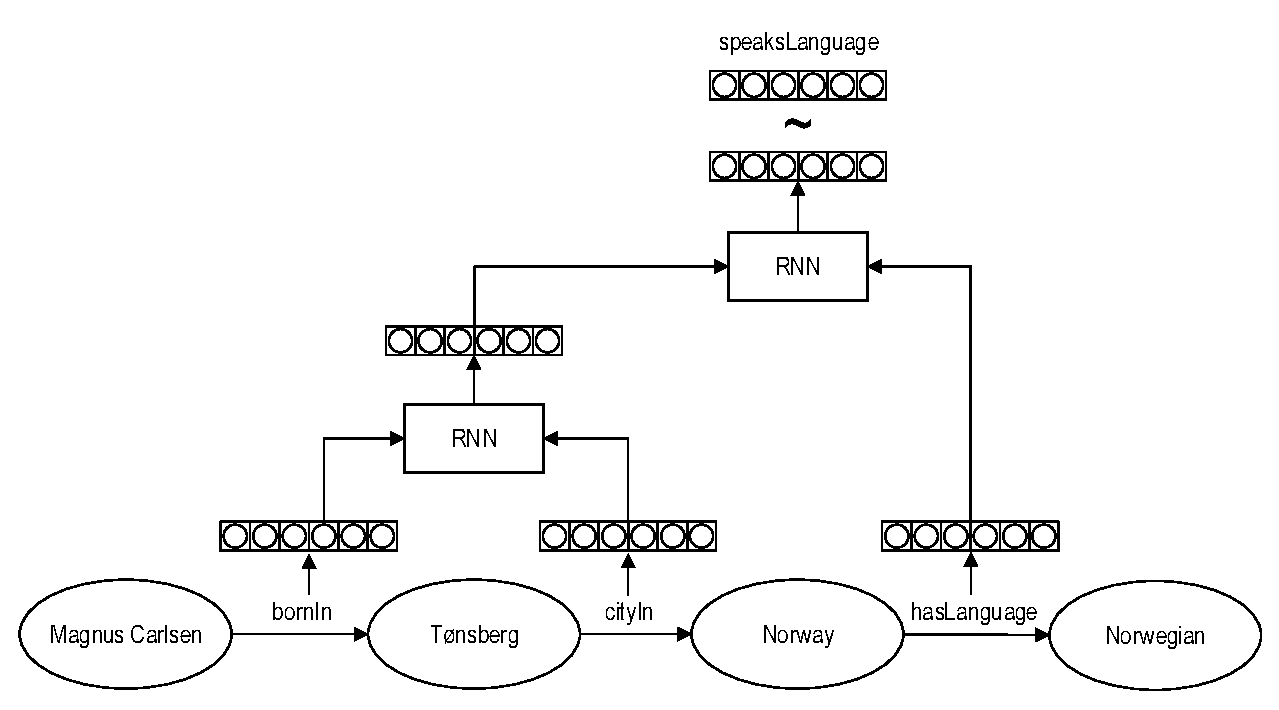
\includegraphics[width=\textwidth]{fig/paths/pathrnn}
%     \caption{Overview of the PATH-RNN method}
%     \label{fig:path-rnn}
% \end{figure}

% \citet{das2017} improve the previously discussed PATH-RNN method with their Single-Model proposal. They point out that taking the embeddings of the entities in a path into account can provide useful information. To represent a path, they recursively combine the embeddings of both the entities and relations in it using RNNs. Furthermore, they propose using a number of different functions to select the best path: \textit{Top-K}, \textit{Average} and \textit{LogSumExp}. They experimentally conclude that the \textit{LogSumExp} function performs better when completing a Knowledge Graph. Figure~\ref{fig:path-single} displays a visual overview of Single-Model. In this Figure, entity embeddings are represented in blue, and relation embeddings in orange. The path that is being considered is the same as in Figure~\ref{fig:path-rnn}.

% \begin{figure}[!htp]
%     \centering
%     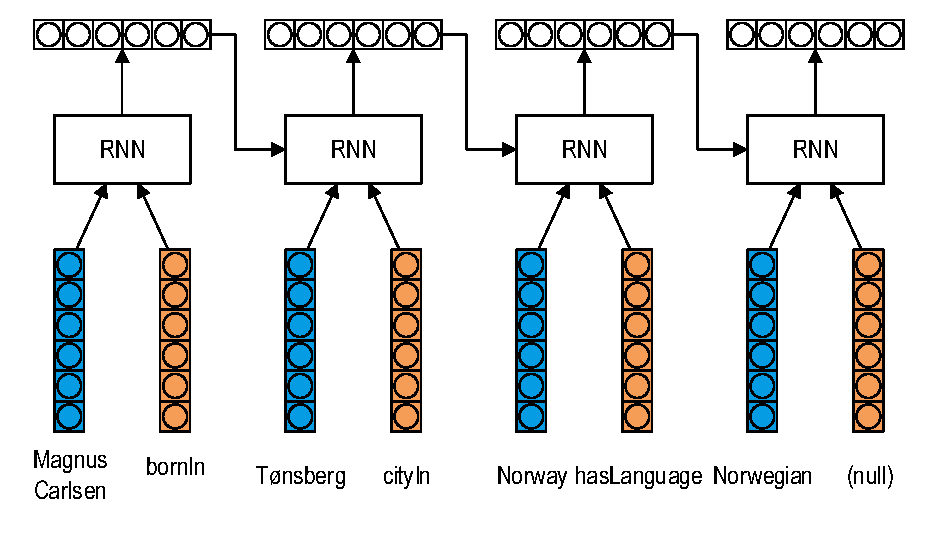
\includegraphics[width=.9\textwidth]{fig/paths/singlemodel}
%     \caption{Overview of the Single-Model method}
%     \label{fig:path-single}
% \end{figure}

% \citet{xiong2018} proposed GMatching, a technique that specializes in extracting information from KG neighborhoods using relatively infrequent relations, which are traditionally considered more challenging due to the reduced amount of information about them present in the graph. GMatching is comprised of two main components: a neighbor encoder, which creates an embedded representation for an entity in a neighborhood; and a matching checker, which computes the similarity of two entity embeddings created by the first component. A visual representation of this proposal is provided in Figure~\ref{fig:path-gmatching}. The meaning of the colors is the same as in the previous Figure.

% \begin{figure}[!htp]
%     \centering
    
%     \subfigure[An example KG]{
%         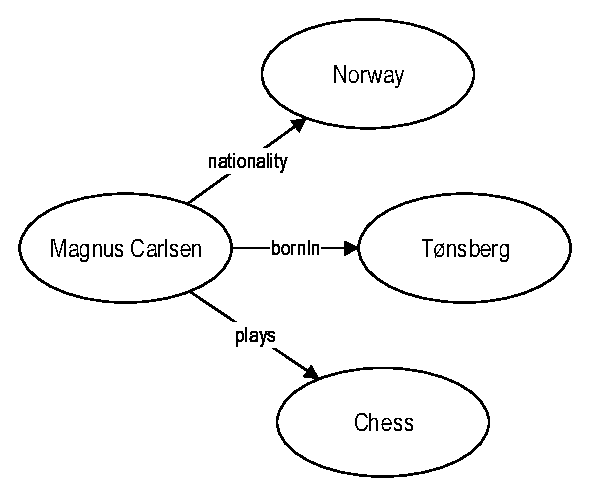
\includegraphics[width=.45\textwidth]{fig/paths/gmatching-a}
%     }\\
%     \subfigure[Encoding of the neighborhood of the entity \textit{Magnus Carlsen}]{
%         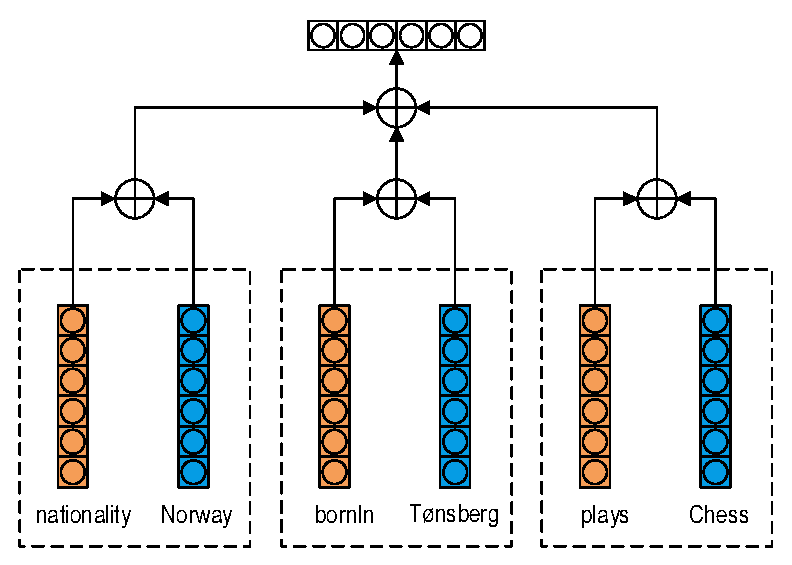
\includegraphics[width=.7\textwidth]{fig/paths/gmatching-b}
%     }

%     \caption{Overview of the GMatching method}
%     \label{fig:path-gmatching}
% \end{figure}

% \citet{shen2017} proposed Implicit ReasoNets (IRNs), a neural network architecture that is able to reason about paths of different lengths in a KG. It is an encoder-decoder model that is governed by a central controller, which allows the whole process to be carried out with no human intervention. Also, it introduces the usage of a shared memory that implicitly stores relevant information about the graph, allowing it to be more efficient and have a smaller memory footprint.

% Additionally, a number of improvements have been made to the baseline translational models to help them leverage path information in several ways. For instance, \citet{lin2015} have proposed PTransE, an extension of TransE that uses path information in its confidence function. Its goal is to give a higher confidence score to those entities that are well-connected together by means of paths that are semantically similar to the relation in the triple that is being evaluated.

% \citet{garcia-duran2015b} proposed RTransE, which represents paths as a series of translations in the embedded space defined by the TransE model. For efficiency reasons, RTransE is limited to using only paths that contain two relations. Likewise, \citet{xiong2018b} introduced PTransD, an enhancement of TransD that performs subsequent translations to model paths. However, PTransD uses two embeddings to represent each entity, to perform operations in parallel.

\section{Explainability?}\label{sec:rl<REPLACE THIS>}
this needs some more classification I`m not sure how yet, maybe when I begin writing it...

% Considering the possible paths between two entities is undoubtedly helpful, but this concept can be expanded further. Rather than a single path, we can consider the entirety of the region of a Knowledge Graph around a certain entity, in other words, its neighborhood. The concept of entity neighborhood is visually shown in Figure~\ref{fig:path-neighborhood}, which depicts the closest and more extended neighborhoods of an entity shown in the center.

% \begin{figure}[!htp]
%     \centering
%     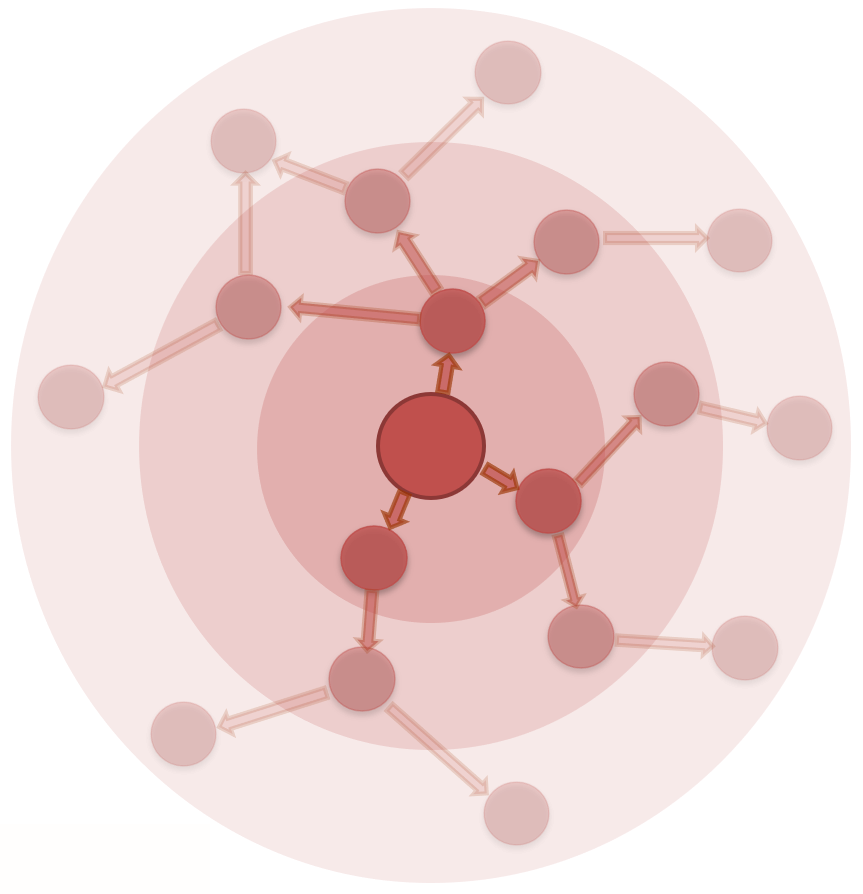
\includegraphics[width=.7\textwidth]{fig/paths/neighborhoods-b.png}
%     \caption{A visual representation of entity neighborhoods}
%     \label{fig:path-neighborhood}
% \end{figure}


% Given a pair of entities, their neighborhoods can be analyzed to determine if a relation should be present between them. This idea has been put to practice by a number of authors.

% \citet{bansal2019a2n} proposed the A2N method, which aggregates the entities in a neighborhood together to obtain a more compact representation of said neighborhood. It uses an attention-based mechanism to focus on the most prominent entities, giving a trustworthy representation of the entities surrounding another one. Additionally, it is designed such that the computational cost of the method does not increase greatly with the size of the neighborhoods.

% The use of attention-based mechanisms in this regard has not gone unnoticed by other authors. \citet{wang2019} have proposed LAN, another approach that aggregates the contents of an entity neighborhood together, however, the attention-based technique that they propose uses weights to give more importance to more relevant entities. \citet{kong2019} also proposes using attention to filter out possibly irrelevant relations in the graph, allowing the models to focus only on more meaningful information, which is especially relevant in the case of heterogeneous Knowledge Graphs. Similarly, \citet{nathani2019} introduced the KBAT method, which is able to capture information from both the entities and the relations in a KG neighborhood. 

% \citet{zhang2020} further the previous idea by adding a weighted attention system to both entities and relations, acknowledging that not all knowledge in the KG is equally useful. Two different attention-based mechanisms are used in their proposal. First, the relation-level attention provides an intuition for which connections from an entity may provide more useful information. Then, the reached entities are considered according to their entity-level attention. This composite, hierarchical attention mechanism allows it to outperform other attention-based proposals.

% \citet{ferre2019} proposes finding missing information by finding similar entities in commonly occurring graph patterns, through the application of concepts of nearest neighbors \cite{denoeux1995}. It does not require any sort of pre-processing of the Knowledge Graph, making it very efficient. Furthermore, its reliance on graph patterns makes it a more interpretable method than other similar proposals.



\section{Summary}\label{sec:path-summary}
The contents of this chapter have provided an overview of the methods to perform Knowledge Graph completion that use relational paths. We have first listed the most prominent scientific proposals that extract paths from a KG and characterize them using features, to learn which paths can be predictive of correct knowledge. Afterwards, we have centered on the proposals that use entity neighborhood information in a number of ways. Finally, we have introduced the approaches that merge together path-based information with latent entity representations, entity and relation embeddings, and neural networks.